\documentclass[10pt,letterpaper]{memoir}
    % memoir commands to define the text block geometry
    \setulmarginsandblock{0.75in}{*}{*}
    \setlrmarginsandblock{0.5in}{*}{*} % leave space in left margin for punched holes

\usepackage{xparse}
\usepackage{blindtext}
\usepackage{xwatermark}
\usepackage{enumitem}
\usepackage{graphicx}
\usepackage{amsmath}

\usepackage{tcolorbox}
    \tcbuselibrary{skins}
\usepackage{pgfplots}
    \pgfplotsset{compat=newest}
\usepackage{tagging}

    \dashundergapssetup{
        gap-format=underline,
        teacher-gap-format=dot,
        gap-font={\ECFAugie\MTversion{augie}\color{black}},
        gap-numbers=false,
        gap-widen=true,
        gap-extend-percent=75, % note: making this too big might create errors
        gap-number-format=\,\textsuperscript{\normalfont(\thegapnumber)},
    }
% ---------------------------------------------------------------------------
% a header to put at the top of a homework assignment
% ---------------------------------------------------------------------------
% #1 class name 
% #2 assignment number (eg, 2.5 CW)
% #3 assignment title (eg, Solve Quadratic Equations)
%
\NewDocumentCommand{\myAssignmentHeader}{ O{Algebra~2} m m }{
    \noindent
    \whenHONORS{Honors~}#1
    \hfill 
    Name : \fbox{\phantom{X\hspace{2in}}}\par
    \vspace{0.5em}
    \noindent
    {%
        \LARGE\sffamily
        \whenHONORS{H-}#2 -- #3
    }
    \hfill
    Period : \fbox{\phantom{\large 9999}}
    \hrule\hspace{\baselineskip}
    \vspace{0.5\baselineskip}
}


% ---------------------------------------------------------------------------
% I'm SO tired of writing these two explicitly!
% ---------------------------------------------------------------------------
\newcommand{\myEmph}[1]{{\bfseries\itshape#1}}

% ---------------------------------------------------------------------------
% For writing TI-84 instructions it's useful to have a visually
% distinct way to format the keys.
% ---------------------------------------------------------------------------
\newcommand{\myKey}[1]{{\ttfamily [#1]}}

\newcommand{\myDesmos}{{\scshape Desmos~}}
\newcommand{\myTi}{{\scshape TI-84~}}

% ---------------------------------------------------------------------------
% Teachers vs. Students ("tstu")
% ---------------------------------------------------------------------------
\newif\iftstu

% Typically, I will set one of these ONCE at the top of the doc.
\newcommand{\forTEACHER}{%
    \tstutrue%
    \dashundergapssetup{teacher-mode=true,}%
}
\newcommand{\forSTUDENT}{%
    \tstufalse%
    \dashundergapssetup{teacher-mode=false,}%
}

% These will conditionally generate output (the argument) based on 
% whether this document is "for" HONORS or ONLEVEL according to the previous commands.
%
% #1 the content 
% #2 text color
\NewDocumentCommand{\whenTEACHER}{ O{red} m }{\iftstu{\ECFAugie\color{#1}#2}\else{}\fi}
\newcommand{\whenSTUDENT}[1]{\iftstu{}\else{#1}\fi}



% ---------------------------------------------------------------------------
% command for creating a 1- or 2-question warmup problem
%
% #1 date
% #2 optional general directions
%
% ---------------------------------------------------------------------------
\NewDocumentEnvironment{myWarmupProblems}{ 
        O{
            \begin{itemize}
                \item Show {\itshape all} your work.
                \item Put a \fbox{box} around your answer.
            \end{itemize}
            \vspace{0.5em}
        } 
    }
{
    \newpage
    {
        \sffamily
        \begin{center}
            {
                \huge\bfseries%
                \whenHONORS{Honors~}Algebra 2 Warmup
            }%
            \\[0.5em]
            {\Large\itshape\printdate}
        \end{center}
        \noindent{\Large#1}
    }
    \large
}{
}


% ---------------------------------------------------------------------------
% A centered tcolorbox
% ---------------------------------------------------------------------------
%
% #1 - optional options to pass to tcolorbox
% #2 - the contents to put in the box
%
\NewDocumentEnvironment{myCenteredBox}{ O{} m }{%
    \begin{center}
        \begin{tcolorbox}[#1]#2\end{tcolorbox}
    \end{center}
}

% ---------------------------------------------------------------------------
% Split the output into two (roughly) equally sized side-by-side minipages.
% ---------------------------------------------------------------------------
%
% #1 - content of first minipage
% #2 - content of second minipage
%
\NewDocumentCommand{\myTwoMinipages}{mm}{
    \begin{minipage}{0.49\textwidth}
        #1
    \end{minipage}
    % \hfill 
    \begin{minipage}{0.49\textwidth}
        #2
    \end{minipage}
}


% ---------------------------------------------------------------------------
% A version of \sqrt 
% ---------------------------------------------------------------------------
%
% #1 index of the root
% #2 uproot amount
% #3 radicand
%
\NewDocumentCommand{\myRoot}{ o O{2} m  }{%
    \IfNoValueTF{#1}{\sqrt{#3\,}}{\sqrt[\uproot{#2}#1]{#3\,}}
}


% ---------------------------------------------------------------------------
% changes to part/chapter/section
% I am piggybacking Units and Lessons on Latex Parts and Chapters, respectively. 
% ---------------------------------------------------------------------------

% Here are some of the macros that capture "my settings".
\newcommand{\myPartName}{Unit}      % what I'll replace "Unit" with.
\newcommand{\myChapterName}{Lesson} % what I'll replace "Chapter" with.
\newcommand{\myLessonSuffix}{}      % a suffix after lesson (chapter) numbers (eg, 'a' in Lesson 5.2a)

% Redefine the Latex part and chapter names to use "my settings".
\renewcommand{\partname}{\myPartName}       % "Unit 2" instead of "Part II"
\renewcommand{\thepart}{\arabic{part}}
\renewcommand{\chaptername}{\myChapterName} % "Lesson 2" instead of "Chapter 2"

% A \chapter-based command to generate a lesson.
% This is a thin wrapper around \chapter that allows me
% to explicitly specify the lesson number. 
%
% #1 lesson name
% #2 optional lesson number (eg, the '2' in Lesson 5.2)
% #3 optional lesson suffix (eg, the 'a' in Lesson 5.2a)
%
\NewDocumentCommand{\myLesson}{ m O{1} O{} }
{
    \setcounter{chapter}{#2-1}
    \renewcommand{\myLessonSuffix}{#3}
    \chapter{#1}
}

% remove chapter numbers from section numbering
\makeatletter
\renewcommand\thesection{\@arabic\c@section}
\makeatother

% simulate a part without typesetting one
% 
% #1 - the part (unit) number
% #2 - the part (unit) title
\newcommand{\dummypart}[2]{%
    \setcounter{part}{#1}
    \partmark{#2}
}

% ---------------------------------------------------------------------------
% These are "annotations", the foundation of the blocked-in-text that I use.
%
% I use the term "annotations" to capture the common
% infrastructure I use to define Objectives, Vobabulary & Concepts.
% ---------------------------------------------------------------------------

% font and styling commands for
% Objectives, Voculary, Key Concepts, etc...
\newcommand{\myAnnotationStyling}{\bfseries\large}

% #1 : name of the kind of annotation (Objectives, ...)
% #2 : title text to go with the annotation
% #3 : extra tcolorbox options
%
\NewDocumentEnvironment{myAnnotate}{ m m O{}}{
    \begin{tcolorbox}[
        colbacktitle=blue!10!white,
        colback=white,
        coltitle=black,
        fonttitle={\myAnnotationStyling},
        title={#1:~},
        after title={\normalfont\itshape#2},
        #3,
        ]
}{
    \end{tcolorbox}
}

% #1 : name of the kind of annotation 
% #2 : title 
%
\NewDocumentEnvironment{myTabularAnnotate}{ m m }{
    \begin{myAnnotate}{#1}{#2}
    \begin{tabular}{r|l}
}{
    \end{tabular}
    \end{myAnnotate}
}
% #1 - column 1 text
% #2 - column 2 text
%
\NewDocumentCommand{\myRow}{mm}{{\bfseries\itshape \textcolor{blue}{#1}}&#2\\[1ex]}

% #1 : name of the kind of annotation 
% #2 : title 
% #3 : text before the list starts
%
\NewDocumentEnvironment{myListAnnotate}{ m m o }{
    \begin{myAnnotate}{#1}{#2}
    \IfValueT{#3}{#3}
    \begin{enumerate}[itemsep=0pt,fullwidth,]
}{
    \end{enumerate}
    \end{myAnnotate}
}
% #1 - column 1 text
% #2 - column 2 text
%
\NewDocumentCommand{\myItem}{mm}{\item{\bfseries\itshape \textcolor{blue}{#1}} #2}


% ---------------------------------------------------------------------------
% A table for systems of equations word problems.
%
% #1 scale factor
% ---------------------------------------------------------------------------
\NewDocumentCommand{\mySystemTable}{O{8}}{
    \begin{center}
        \begin{tabular}{|m{5em}|m{2in}|m{2in}|m{1.5in}|}
            \hline
            {\bfseries\itshape variables} & {\bfseries\itshape equations} & {\bfseries\itshape system} & {\bfseries\itshape augmented matrix} \\
            \hline\hline
            \scalebox{#1}{\fontsize{32pt}{0pt}\selectfont \phantom{\textbf{I}}} & \phantom{X} & \phantom{X} & \phantom{X}\\
            \hline
        \end{tabular}
    \end{center}
}

\NewDocumentCommand{\myBetterSystemTable}{O{4}}{
    \begin{center}
        \begin{tabular}{|m{3.25in}|m{3.25in}|}
            \hline
            \underline{\bfseries\itshape variables:} & \underline{\bfseries\itshape system of equations:}  \\
            \scalebox{#1}{\fontsize{32pt}{0pt}\selectfont \phantom{\textbf{I}}} & \phantom{X} \\
            \hline
            \underline{\bfseries\itshape augmented matrix:} & \underline{\bfseries\itshape RREF matrix:} \\
            \scalebox{#1}{\fontsize{32pt}{0pt}\selectfont \phantom{\textbf{I}}} & \phantom{X} \\
            \hline
        \end{tabular}
    \end{center}
}
\usepackage{xparse}
\usepackage{blindtext}
\usepackage{xwatermark}
\usepackage{enumitem}
\usepackage{graphicx}
\usepackage{amsmath}

\usepackage{tcolorbox}
    \tcbuselibrary{skins}
\usepackage{pgfplots}
    \pgfplotsset{compat=newest}
\usepackage{tagging}

    \hypersetup{pdfborder = {0 0 0}} % so the box doesn't show up in the footnote link
% ---------------------------------------------------------------------------
% x-y graphs using Tkz
% ---------------------------------------------------------------------------

% a simple "symmetric" x-y graph
%
% #1 scale of the full graph
% #2 max/min x
% #3 max/min y (optional, if absent it defaults to the x argument)
%
\NewDocumentCommand{\mySymmetricGraph}{ O{0.5} m o }{
    \begin{tikzpicture}[
        scale=#1,
        xaxe style/.style = { very thick, arrows={-{Straight Barb}}, },                 
        yaxe style/.style = { very thick, arrows={-{Straight Barb}}, },                 
        ]
        \tkzInit[
            xmax=#2, xmin=-#2, xstep=1,
            ymax=\IfValueTF{#3}{#3}{#2}, ymin=-\IfValueTF{#3}{#3}{#2}, ystep=1,
            ]
        \tkzGrid[ sub, subxstep=1, subystep=1, ]
        \tkzDrawX[label={$x$},color=black, right=0.2em,]
        \tkzDrawY[label={$y$},color=black, above=0.2em,]
        % \tkzLabelX[orig=false,]
        % \tkzLabelY[orig=false,]
        % \tkzFct[{-(},solid,very thick,color=black,samples=50,domain =-6:6.5]{\x}
    \end{tikzpicture}
}
% A counter to number the problems in the guided notes.
\newcounter{MyProblemCounter}
\setcounter{MyProblemCounter}{1}
\newcommand{\useMyProblemCounter}{\theMyProblemCounter\stepcounter{MyProblemCounter}}


\newcommand{\myProblemFont}{\bfseries\itshape}



% ---------------------------------------------------------------------------
% These are the commands I use to format the problems in the guided notes
% that have an empty space where I will write during class.
% ---------------------------------------------------------------------------

% A single problem that takes half the page.
%
% #1 : optional directions for the problem(s)
% #2 : details for problem 1
% #3 : optional font style for box titles
% #4 : vertical height of the problem boxes
% #5 : optional text at the bottom
%
\NewDocumentCommand{\myProblem}{ o m O{\large} m O{} }{%
    \IfValueT{#1}{\vspace{1\parskip}\noindent#1\nopagebreak}%
    \begin{tcbraster}[%
        raster equal height,%
        raster columns=2,%
        raster column skip=0.5mm,%
        raster row skip=0.5mm,%
        ]%
        % This is the first problem.
        \begin{tcolorbox}[%
            enhanced,%
            sharp corners,%
            colback=white,%
            coltitle=black, colbacktitle=black!10!white,%
            boxrule=0pt, borderline={0.5pt}{0pt}{black},%
            title={\texttt{\useMyProblemCounter}},%
            attach boxed title to top left%
            ]
            #3#2
            \tcblower\vspace{#4}#5
        \end{tcolorbox}
        %
        % There IS no second problem. So make it empty space.
        \begin{tcolorbox}[colback=white, colframe=white,]\end{tcolorbox}%
    \end{tcbraster}
}

% A single problem that takes the full width of the page.
%
% #1 : optional directions for the problem(s)
% #2 : details for problem 1
% #3 : optional font style for box titles
% #4 : vertical height of the problem boxes
% #5 : optional text at the bottom
%
\NewDocumentCommand{\myWideProblem}{ o m O{\large} m O{} }{%
    \IfValueT{#1}{\vspace{1\parskip}\noindent#1\nopagebreak}%
    \begin{tcbraster}[%
        raster equal height,%
        raster columns=1,%
        raster column skip=0.5mm,%
        raster row skip=0.5mm,%
        ]%
        % This is the first problem.
        \begin{tcolorbox}[%
            enhanced,%
            sharp corners,%
            colback=white,%
            coltitle=black, colbacktitle=black!10!white,%
            boxrule=0pt, borderline={0.5pt}{0pt}{black},%
            title={\texttt{\useMyProblemCounter}},%
            attach boxed title to top left%
            ]
            #3#2
            \tcblower\vspace{#4}#5
        \end{tcolorbox}
    \end{tcbraster}
}

% Two problems next to each other.
%
% #1 : optional directions for the problem(s)
% #2 : details for problem 1
% #3 : details for problem 2
% #4 : optional font style for box titles
% #5 : vertical height of the problem boxes
% #6 : optional text at the bottom of problem 1
% #7 : optional text at the bottom of problem 2
%
\NewDocumentCommand{\myProblems}{ o m m O{\large} m O{} O{#6} }{%
    \IfValueT{#1}{\vspace{1\parskip}\noindent#1\nopagebreak}%
    \begin{tcbraster}[%
        raster equal height,%
        raster columns=2,%
        raster column skip=0.5mm,%
        raster row skip=0.5mm,%
        ]%
        % This is the first problem.
        \begin{tcolorbox}[%
            enhanced,%
            sharp corners,%
            colback=white,%
            coltitle=black, colbacktitle=black!10!white,%
            boxrule=0pt, borderline={0.5pt}{0pt}{black},%
            title={\texttt{\useMyProblemCounter}},%
            attach boxed title to top left%
            ]
            #4#2
            \tcblower\vspace{#5}#6
        \end{tcolorbox}
        % This is the second problem. 
        \begin{tcolorbox}[%
            enhanced,%
            sharp corners,%
            colback=white,%
            coltitle=black, colbacktitle=black!10!white,%
            boxrule=0pt, borderline={0.5pt}{0pt}{black},%
            title={\texttt{\useMyProblemCounter}},%
            attach boxed title to top left%
            ]
            #4#3
            \tcblower\vspace{#5}#7
        \end{tcolorbox}
    \end{tcbraster}
}

% ---------------------------------------------------------------------------
% These are the commands I use to format the problems in the guided notes
% that have an partially filled space where I will also write during class.
%
% I use the term "with content" to refer to this partially filled space.
% ---------------------------------------------------------------------------

% A single problem that takes half the page.
%
% #1 : optional directions
% #2 : the problem contents
% #3 : optional font style for the content
%
\NewDocumentCommand{\myProblemWithContent}{ o m O{\large} }{%
    \IfValueT{#1}{\vspace{1\parskip}\noindent#1\nopagebreak}%
    \begin{tcbraster}[%
        raster equal height,%
        raster columns=2,%
        raster column skip=0.5mm,%
        raster row skip=0.5mm,%
        ]%
        % This is the first problem.
        \begin{tcolorbox}[%
            enhanced,%
            sharp corners,%
            colback=white,%
            coltitle=black, colbacktitle=black!10!white,%
            boxrule=0pt, borderline={0.5pt}{0pt}{black},%
            title={\texttt{\useMyProblemCounter}},%
            attach boxed title to top left%
            ]
            #3#2
        \end{tcolorbox}
        %
        % There IS no second problem. So make it empty space.
        \begin{tcolorbox}[colback=white, colframe=white,]\end{tcolorbox}%
    \end{tcbraster}
}


% Two problems that that sit next to each other.
%
% #1 : optional directions
% #2 : the 1st problem contents
% #3 : the 2nd problem contents
% #4 : optional font style for the content
%
\NewDocumentCommand{\myProblemsWithContent}{ o m m O{\large} }{%
    \IfValueT{#1}{\vspace{1\parskip}\noindent#1\nopagebreak}%
    \begin{tcbraster}[%
        raster equal height,%
        raster columns=2,%
        raster column skip=0.5mm,%
        raster row skip=0.5mm,%
        ]%
        % This is the first problem.
        \begin{tcolorbox}[%
            enhanced,%
            sharp corners,%
            colback=white,%
            coltitle=black, colbacktitle=black!10!white,%
            boxrule=0pt, borderline={0.5pt}{0pt}{black},%
            title={\texttt{\useMyProblemCounter}},%
            attach boxed title to top left%
            ]
            #4#2
        \end{tcolorbox}
        % This is the second problem.
        \begin{tcolorbox}[%
            enhanced,%
            sharp corners,%
            colback=white,%
            coltitle=black, colbacktitle=black!10!white,%
            boxrule=0pt, borderline={0.5pt}{0pt}{black},%
            title={\texttt{\useMyProblemCounter}},%
            attach boxed title to top left%
            ]
            #4#3
        \end{tcolorbox}
    \end{tcbraster}
}


% A wide problem that can have any latex code in the content area of the box.
%
% #1 : optional directions 
% #2 : the problem
% #3 : optional font style for the content
%
\NewDocumentCommand{\myWideProblemWithContent}{ o m O{\large} }{%
    \IfValueT{#1}{\vspace{1\parskip}\noindent#1\nopagebreak}%
    \begin{tcbraster}[%
        raster equal height,%
        raster columns=1,%
        raster column skip=0.5mm,%
        raster row skip=0.5mm,%
        ]  
        \begin{tcolorbox}[%
            enhanced,%
            sharp corners,%
            colback=white,%
            coltitle=black, colbacktitle=black!10!white,%
            boxrule=0pt, borderline={0.5pt}{0pt}{black},%
            title={\texttt{\useMyProblemCounter}},%
            attach boxed title to top left%
            ]%
            #3#2
        \end{tcolorbox}
    \end{tcbraster}
}

\forHONORS
\forSTUDENTorTEACHER % which one? it depends on an env. var. (defined in the build recipe)



\begin{document}
\pagestyle{plain}
\checkandfixthelayout
\raggedbottom

\setlength{\parskip}{1\onelineskip}
\setlength{\parindent}{0in}

%-----------------------------------------------------------------------------------------
\myAssignmentHeader{9.6 HW}{Overfitting Scatterplot Data}
%-----------------------------------------------------------------------------------------

In the last lesson, we added rational expressions. 
We simplified expressions that looked like this.
\[
    \frac
    {(x-2)}
    {(x+3)}
    +
    \frac
    {3x}
    {(x+3)(x+5)}
\]
%
Today we will subtract like this:
\[
    \frac
    {(x-2)}
    {(x+3)}
    \bm{-}
    \frac
    {3x}
    {(x+3)(x+5)}
\]


\begin{tcolorbox}[center,colback=white,width=7in,]
    {\bfseries\itshape Subtraction} 
    is mostly the same as addition.
    The key idea is to combine the fractions 
    over a common \gap{denominator} (LCD).\par
    \vspace{1em}
    But for subtraction, 
    you need to remember to \gap{distribute} the negative.
    This is easy to forget!
\end{tcolorbox}

\begin{myConceptSteps}{To {\bfseries\itshape subtract} two rational expressions\dots}
    \myStep{common denominator}{
        If the fractions have \gap{different} denominators\dots
        \begin{itemize}[nosep]
            \item Factor the denominators.
            \item Find the \gap{LCD} of the two rational expressions.
            \item \gap{Multiply} the numerators and denominators 
            by factors needed to make their denominators equal to the \gap{LCD}.
        \end{itemize}
    }
    \myStep{subtract}{%
        Subtract the \gap{numerators}.
        \begin{itemize}[nosep]
            \item{\bfseries\itshape Do not} subtract the denominators.
            The denominator becomes the \gap{LCD}. 
        \end{itemize}
    }
    \myStep{simplify}{%
        Simplify the expression.
        \begin{itemize}[nosep]
            \item Remember to \gap{distribute} the negative. 
        \end{itemize}
    }
\end{myConceptSteps}


\myWideProblem
    {
        $
        \frac{2x}{x^2+2x-8}
        -
        \frac{1}{2}
        $
    }
    {6.5in}
\section{Polynomial Long Division}

\begin{myConcept}{~To divide polynomials by long division \dots}
    \begin{center}
        \begin{tabular}{m{0.5\textwidth}|p{0.45\textwidth}}
            & 
            {\Large $ \frac{2x^2  -1}{x-3} $}
            \rule{0in}{1\baselineskip}
            \\ \hline
            {\bfseries\itshape Step 1.}
            Write the dividend and divisor
            as a long division problem.
            Write the polynomials in {\bfseries\itshape descending order}.
            Fill in {\bfseries\itshape zeros} for missing terms. 
            & 
            \rule{0in}{2\baselineskip}
            \\ \hline
            {\bfseries\itshape Step 2.}
            Divide the {\bfseries\itshape leading term} in the dividend 
            by the {\bfseries\itshape leading term} in the divisor.
            Write this above the dividend.
            & 
            \rule{0in}{4\baselineskip}
            \\ \hline
            {\bfseries\itshape Step 3.}
            Multiply the divisor by this expression (distribute).
            Write the new terms {\bfseries\itshape lined up} under the dividend.
            & 
            \rule{0in}{4\baselineskip}
            \\ \hline
            {\bfseries\itshape Step 4.}
            {\bfseries\itshape Subtract} to form a new polynomial.
            & 
            \rule{0in}{7\baselineskip}
            \\ \hline
            {\bfseries\itshape Step 5.}
            {\bfseries\itshape Repeat} with the new polynomial.
            & 
            \rule{0in}{9\baselineskip}
            \\ \hline
            {\bfseries\itshape Step 6.}
            Stop when there is nothing left to bring down.
            The {\bfseries\itshape quotient} is the polynomial above the dividend.
            Write the {\bfseries\itshape remainder} as a fraction over the divisor.
            & 
            \\ 
        \end{tabular}
    \end{center}
\end{myConcept}

\myProblems[Divide these polynomials.]
    {
        $
            (3x^3 - 8x^2 - 13x + 9) 
            \div
            (3x+4)
        $
    }
    {
        \Large
        $\frac
            {2x^4 - 5x^2 - 2x - 11} 
            {x^2 - 4}
        $
    }
    {5in}

\section{Transformations Cheat Sheet}

\begin{tcolorbox}[center,colback=white,width=3.5in,valign=center,]
{
    \vspace{-0.9\onelineskip}
    \begin{equation*}
        f(x)=b^x \text{\quad\huge$\rightarrow$\quad} g(x) = \bm{a} \, b^{x - \bm{h}} + \bm{k}
    \end{equation*}
}
\end{tcolorbox}
\begin{myWarningBox}
    \begin{center}
        Remember that $\bm{h}$ is the \gap{opposite} 
        of what you see in the formula for $g(x)$.
    \end{center}
\end{myWarningBox}


{
\small 
\begin{tcbraster}[
    raster columns = 2,
    raster equal height,
    colback = white,
    % raster left skip = 0.75in, raster right skip = 0.75in, raster column skip = 0.75in,
    % raster before skip = 0.25in, raster after skip = 0.25in,
]
    \begin{tcolorbox}[
        title=Transformations, 
        coltitle=black, 
        colbacktitle=black!20, 
        fonttitle=\sffamily\bfseries\centering\large,
        boxrule=0.5pt,
        ]
        \centering
        \renewcommand{\arraystretch}{1.75}
        % {\small $|\bm{a}|, |\bm{h}|, |\bm{k}|$ \itshape mean \gap{ignore} the sign}
        \begin{tabular}[t]{|>{\raggedright}p{1in}|p{1.75in}|}
            \hline
            {\itshape vertical} {\bfseries\itshape reflection} 
            & if $\bm{a}$ is \gap{negative}\\ 
            % & \\
            % & \\
            \noalign{\hrule height 0.25pt}
            {\itshape vertical} {\bfseries\itshape stretch} by $|\bm{a}|$
            &  if $|\bm{a}|$  is \gap{$> 1$} \\ 
            % & \\
            % & \\
            \noalign{\hrule height 0.25pt}
            {\itshape vertical} {\bfseries\itshape compression} by $|\bm{a}|$
            &  if $|\bm{a}|$ is \gap{$< 1$} \\ 
            % & \\
            % & \\
            \noalign{\hrule height 1.5pt}
            {\itshape horizontal shift} {\bfseries\itshape right} by $|\bm{h}|$
            &  if $\bm{h}$  is \gap{positive}\\ 
            % & \\
            % & \\
            \noalign{\hrule height 0.25pt}
            {\itshape horizontal shift} {\bfseries\itshape left} by $|\bm{h}|$
            &  if $\bm{h}$  is \gap{negative}\\ 
            % & \\
            % & \\
            \noalign{\hrule height 1.5pt}
            {\itshape vertical shift} {\bfseries\itshape up} by $|\bm{k}|$
            &  if $\bm{k}$  is \gap{positive}\\ 
            % & \\
            % & \\
            \noalign{\hrule height 0.25pt}
            {\itshape vertical shift} {\bfseries\itshape down} by $|\bm{k}|$
            &  if $\bm{k}$  is \gap{negative}\\ 
            % & \\
            % & \\
            \hline
        \end{tabular}
    \end{tcolorbox}
    \begin{tcolorbox}[
        title=Attributes, 
        coltitle=black, 
        colbacktitle=black!20, 
        fonttitle=\sffamily\bfseries\centering\large,
        boxrule=0.5pt,
        ]
        \centering
        \renewcommand{\arraystretch}{1.145}
        \begin{tabular}[t]{|>{\raggedright}p{0.75in}|p{2in}|}
            \hline
            {\bfseries\itshape G or D?} & if {$b>1$}: \whenTEACHER{growth}\\
            {}                                  & if {$0<b<1$}: \whenTEACHER{decay}\\
            % {} & \\
            \noalign{\hrule height 1.5pt}
            \hline
            {\bfseries\itshape horiz. asymp.} & \whenTEACHER{$y=k$}\\
            & \\
            \noalign{\hrule height 1.5pt}
            {\bfseries\itshape domain} & \whenTEACHER{all real numbers}\\
            % & \\
            \noalign{\hrule height 1.5pt}
            {\bfseries\itshape range} & if {$\bm{a}>0$}:\\
            {}                        & \whenTEACHER{$y > k$}\\
            % {}                        & \\
            {} & if {$\bm{a}<0$} (reflected):\\
            {} & \whenTEACHER{$y < k$}\\
            % {} & \\
            \noalign{\hrule height 1.5pt}
            {\itshape\bfseries end beh.} & if {$\bm{a}>0$}:  \\
            & \quad L: \whenTEACHER{as x{$\rightarrow-\infty$}, y{$\rightarrow 0$}}\\
            & \quad R: \whenTEACHER{as x{$\rightarrow+\infty$}, y{$\rightarrow+\infty$}}\\
            % & \\
            &  if {$\bm{a}<0$} (reflected): \\
            & \quad L: \whenTEACHER{as x{$\rightarrow-\infty$}, y{$\rightarrow 0$}}\\
            & \quad R: \whenTEACHER{as x{$\rightarrow+\infty$}, y{$\rightarrow-\infty$}}\\
            % {} & \\
            \hline
        \end{tabular}
    \end{tcolorbox}
\end{tcbraster}

}
\newpage
\section{Evaluating Absolute Value Functions}

\begin{tcolorbox}[center,width=6.5in,colback=white,]
    To evaluate a \gap{function} with absolute values, 
    you just \gap{evaluate} the expression for the function 
    at the input value.
\end{tcolorbox}


\myProblems[Evaluate these functions at the given input value.]
{ 
    $
        f(x) =
        |2x|
    $
    \qquad
    Find $f(6)$.
}
{
    $
        g(x) =
        3|-5x|
    $
    \qquad
    Find $g(30)$.
}
{8\onelineskip}

\myProblems
{
    $
        t(z) =
        |z - 8|
    $
    \qquad
    Find $t(2)$.
}
{
    $
        s(w) =
        1 - 2\left|w + 3\right|
    $
    \qquad
    Find $s(-5)$.
}
{8\onelineskip}


\myProblems[Find the values of $a$, $h$, $k$ in the following transformed reciprocal functions.]
{
    $g(x) = \frac{1}{x-2} + 3$
}
{
    $g(x) = \frac{5}{x+7} - 11$
}
{1.25in}

\myProblems
{
    $g(x) = \frac{-8}{x+7} + 9$
}
{
    $g(x) = \frac{-1}{x+7} - 1$
}
{1.25in}

\myProblems
{
    $g(x) = \frac{2}{4(x+5)} $
}
{
    $g(x) = -\frac{5}{3x} - 3 $
}
{1.25in}

\section*{Fitting a Quintic Model}

Use \myDesmos to find a \myEmph{quintic} {(5th degree)} regression model. 
To do this, use the \myDesmos commands in the table above. 

\myProblemsWithContent
{
    Find the model parameters listed below.
    \begin{center}
        \renewcommand{\arraystretch}{1.4}
        \begin{tabular}{r|l|c}
            model & best fit parameters & $r^2$ or $R^2$ \\ 
            \midrule
            {\itshape Quintic} 
            & $\bm{a_5} =$ \underline{\hspace{0.45in}} $\bm{d_5} =$ \underline{\hspace{0.45in}} & $R^2 =$ \underline{\hspace{0.45in}} \\
            & $\bm{b_5} =$ \underline{\hspace{0.45in}} $\bm{f_5} =$ \underline{\hspace{0.45in}}& \\
            & $\bm{c_5} =$ \underline{\hspace{0.45in}} $\bm{g_5} =$ \underline{\hspace{0.5in}}& \\
        \end{tabular}
    \end{center}
}
{  
    Compare $R^2$ to the previous problems. Is this better or worse?
    Explain your thinking \myEmph{as a full sentence}.
}[\small]

\myProblemsWithContent
{
    Sketch a scatterplot of the $(x,y)$ data. 
    Then sketch the curve 
    $y = \bm{a_5} + \bm{b_5}x + \bm{c_5}x^2 + \bm{d_5}x^3 + \bm{f_5}x^4 + \bm{g_5}x^5$ 
    based on \myDesmos.\newline
        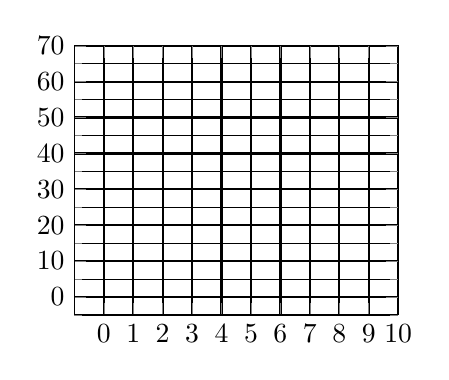
\begin{tikzpicture}
            \begin{axis}[
                scale=0.6,
                grid = both,
                xmin=-1, xmax=10, xtick distance=1, xtickmin=0,
                ymin=-5, ymax=70, ytick distance=10, minor y tick num=1,
                major grid style={solid,thick,black},
                minor grid style={solid,very thin,black},
            ]
            \end{axis}
        \end{tikzpicture}
}
{
    How many points does the curve go through?
}[\small]
\section{Pay It Forward}

\begin{itemize}
    \item The number of people (from the video about Trevor) is a geometric sequence.
    \item Fill in the missing terms.
    
    \begin{tikzpicture}[auto, bend left=30]
        \dashundergapssetup{
            gap-widen=false,
        }
    
        \node (1) at (0,0)  [myShape,draw] {1};
        \node (2) at (2,0)  [myShape,draw] {3};
        \node (3) at (4,0)  [myShape,draw] {9};
        \node (4) at (6,0)  [myShape,draw] {\tiny\gap{27}};
        \node (5) at (8,0)  [myShape,draw] {\tiny\gap{81}};
        \node (6) at (10,0) [myShape,draw] {\tiny\gap{243}};
        \node (dots) at (11.5,0) {\huge\dots};
    
        \draw [-Stealth] (1.north east) to node  {\tiny$\times 3$} (2.north west);
        \draw [-Stealth] (2.north east) to node  {\tiny$\times 3$} (3.north west);
        \draw [-Stealth] (3.north east) to node  {\tiny$\times 3$} (4.north west);
        \draw [-Stealth] (4.north east) to node  {\tiny$\times 3$} (5.north west);
        \draw [-Stealth] (5.north east) to node  {\tiny$\times 3$} (6.north west);
    \end{tikzpicture}  

    \item For this sequence, the first term is $a=$\gap{1}, and the ratio is $r=$\gap{3}.
    
    \item The explicit formula for a geometric sequence is $x_n = a r^{n-1}$. 
    So for Trevor's sequence, the explicit formula is
    \[ x_n = \text{\gap{$3^{n-1}$}} \]

    \item So Trevor's sequence looks like this.
    
    \begin{tikzpicture}[auto, bend left=30]
        \dashundergapssetup{
            gap-widen=false,
        }
    
        \node (1) at (0,0)  [myShape,draw] {$3^0$};
        \node (2) at (2,0)  [myShape,draw] {$3^1$};
        \node (3) at (4,0)  [myShape,draw] {$3^2$};
        \node (4) at (6,0)  [myShape,draw] {$3^3$};
        \node (5) at (8,0)  [myShape,draw] {$3^4$};
        \node (6) at (10,0) [myShape,draw] {$3^5$};
        \node (dots) at (11.5,0) {\huge\dots};
    
        \draw [-Stealth] (1.north east) to node  {\tiny$\times 3$} (2.north west);
        \draw [-Stealth] (2.north east) to node  {\tiny$\times 3$} (3.north west);
        \draw [-Stealth] (3.north east) to node  {\tiny$\times 3$} (4.north west);
        \draw [-Stealth] (4.north east) to node  {\tiny$\times 3$} (5.north west);
        \draw [-Stealth] (5.north east) to node  {\tiny$\times 3$} (6.north west);
    \end{tikzpicture}  

    \item What is the next term in that sequence? \gap{$3^6$}.
    
    \item A name for this sequence is ``powers of \gap{3}''.
\end{itemize}


\end{document}